%---------------------------------------------------------------------------- 
\chapter{Hívásfelépítés Kubernetes nélkül}
%---------------------------------------------------------------------------- 

Ahhoz, hogy a valóshoz hasonló infrastruktúrát lehessen létrehozni, több 
számítógépet kellett valahogyan összekapcsolni és rajtuk a megfelelő szoftvereket
elindítani. A környezet megvalósításához egy VirtualBox nevezetű virtuális gépeket
létrehozó és kezelő alkalmazást választottam. Indoka a választásomnak azon
alapult, hogy egyszerű használni és ingyenes.

De csak a virtuális gépek jelenléte még nem jelenti azt, hogy ezek tudnak egymással
kommunikálni. Ezért a telepítés során csak sima Brideged adapter használtam minden
virtuális gép esetében, ami kiszolgáló számítógép hálózati kártyáján keresztül
képes elérni az internetet. Ezzel hálózattal tökéletesen lehetett tesztelni
akkor, ha az rtpengine nem Kubernetes környezetben működött. Később át kellett
térnem kiszolgáló adapteres hálózat használatára különben a lokális Kubernetes 
fürtöt nem látták a SIP kliensek. 

A kliensek tekintetében is az ingyenességre és az egyszerű használatra törekedtem, 
de fontos volt még az a szempont is, hogy lehessen parancssorosan hívást kezdeményezni
és fogadni. Ezekkel az a funkciókkal rendelkezett a Linphone nevezetű kliens, ami
rendkívül sok beállítást engedélyez ingyenesen a felhasználóinak. Számomra a következő
funkciók voltak nagyon hasznosnak: wav fájl lejátszása hívás közben, használt kódolás
kiválasztása és a hívás rögzítése. A wav fájl lejátszása, azért egy fontos funkció, mert
így nem kell törődni azzal, hogy a mikrofon keresztül valamilyen hangot tudjon rögzíteni.

Egy általános VoIP híváshoz szükség van legalább egy SIP szerverre, ami képes a felhasználókhoz
kapcsolatos információkat kezelni. Erre a célra Kamailio-t használok, mivel ehhez készítették
az rtpeninge-t. Így kézenfekvő volt a használata, de elméletileg lehet más SIP szervereket
is használni az rtpengine-l. A másik fontos, de egyértelmű tényező az maga az rtpengine, 
amiről a következő fejezetben lesz részletesen szó. 

\section{rtpengine}

Az rtpengine egy Sipwise  által fejlesztett a Kamailio-hoz szánt RTP 
proxy, ami nem csak forgalmat képes irányítani, hanem a beérkező csomagokat transzformálni is.
Emellett olyan funkciókkal is rendelkezik, amikkel tudjuk a hívások minőségét monitorozni, 
rendelkezésre állóságát és biztonságát növelni. A következő funkciókat érdemes 
jobban kifejteni: 

\begin{itemize}
	\item Tud IPv4 és IPv6 címeket kezelni és közöttük média forgalmat továbbítani. 
	\item Állítható port tartomány. 
	\item Több interfész használata. 
	\item Kernel szintű csomagtovábbítás a kisebb késleltetés és processzor használat miatt.
	\item HTTP, HTTPS és WebSocket interfész támogatottság.
	\item Médiafolyamok felvétele. 
	\item Híváshoz szükséges statisztikák számítása.
	\item Transzkódolás és újracsomagolás.
	\item SDP csomagok teljesen újraírása. 
\end{itemize}

\subsection{Kernel és felhasználói tér}

Az rtpengine alapvetően a felhasználói térben működik így ilyenkor mindent ott csinál, ami
magasabb késeltetést és processzor használatot igényel. Az oka ennek, hogy mikor egy csomag
érkezik a hálózati interfészre az áthalad a kernelen a fájlleíróig. Ha odajutott egy 
csomag, akkor a hozzá kapcsolódó folyamatot értesíti, ami ebben az esetben az rtpengine, hogy
van mit leolvasni onnét. Ennek során a csomag átkerül a kernelből a felhasználói térbe és 
ami egy nagyon drága művelet. Ha feldolgozásra került a csomag, akkor ugyanezen az útvonalon
fog kimenni. Ez azért nagy probléma, mert az RTP protokoll UDP-t használ és így rengeteg 
kis csomag érkezik folyamatosan, ami nagy terhelést jelent a szerver számára. 

Ezzel szemben, ha használjuk a megfelelő modult, akkor a beérkező csomagok nem kerülnek át a 
felhasználói térbe így kevesebb erőforrás kerül felhasználásra. Ezt úgy éri el az rtpengine,
hogy egy hívás kiépítése során \textbf{iptables} szabályokat hoz létre, amikben definiálja, hogy
adott portra érkező forgalom hova legyen továbbítva. 

Az \textbf{iptables} egy olyan eszköz, amivel a linux kernelben lehet létrehozni 
táblákat szabályokkal, amik IP szinten képesek szűrni a forgalmat. 

%A választás azért erre a proxy-ra esett, mert folyamatos támogatottsága van, sok helyen 
%használják illetve sok olyan funkcióval rendelkezik, ami a projekt szempontjából fontos.

%Ilyen és legszükségesebb funkciója a Redis támogatottsága, amivel egyes hívásokhoz 
%lehet minden szükséges adatot elmenteni és ezen adatok alapján más rtpengine példányok 
%tudják frissíteni a hívásaikat. Így, ha egy az egyik szerver megáll és nem tudja tovább
%kezelni a hívásokat, akkor egy terhelés elosztó áttudja irányítani az összes hívást 
%más szerverekhez, amik ezáltal rendelkeznek a híváshoz szükséges információkkal. 
%
%A Redis támogatottság már létezett, viszont csak akkor, ha az rtpengine konfigurálásánál
%pontosan ismerjük az összes többi rtpengine címét. Alapesetben ezek az információk 
%rendelkezésre állnak, viszont Kubernetes környezetben ezek mind változékonyak. Sosem 
%tudjuk pontosan megjósolni, hogy egy kapszula, ami egy rtpengine szervert futtat milyen
%címmel fog létrejönni. 
%
%Ezt a problémát orvosolta részben Oded Arbell, aki egy Pull Request keretein belül 
%benyújtott egy nulla tudású Redis skálázhatóság funkciót. Mint a neve is utal rá 
%ezzel a megoldással úgy lehet az infrastruktúrába új rtpengine szervereket felvenni, 
%hogy nem kell ismerni a többi résztvevő szerver címét. De ez még mindig csak részben 
%oldotta meg a problémát ugyanis ha van két rtpengine szerverünk, akkor az egyikhez 
%beérkező hívásnál csak azon a szerveren fognak kinyílni a megfelelő portok, amire a 
%hívás beérkezett. Így, ha ez a szerver leáll, akkor a másik nem tudja kezelni a forgalmat,
%mert nincs nyitva egyik szükséges portja sem. 
%
%Megoldásképpen egy kicsit bele kellett nyúlnom ebbe a kódba és beállítani, hogy frissítésnél
%nyisson ki minden olyan portot, ami a hívás információi között szerepel. Így elértem 
%egy olyan fajta redundanciát, amivel a fentebb leírt váltás jól működik. \\
%
%Amit még érdemes megemlíteni, hogy az rtpengine képes kettő különböző módban működni.
%Tud simán a felhasználói névtérben futni, amikor a transzkódolást és az adatok 
%továbbítását is ott végzi el és tudja a kernel névteret is használni, amikor a 
%továbbítást a kernel névtérben végzi. Így processzor erőforrást lehet spórolni, mert
%nem kell a szervernek azt a drága műveletet minden csomagnál elvégeznie, hogy 
%a kernel névtérből felhasználóiba teszi át a csomagokat. 

\subsection{Transzkódolás}

Transzkódolás alatt azt a folyamatot értjük, amikor egy adott formátumú videó- vagy 
hanganyag egy másik formátumba való átalakítása történik. Ezt jelenleg az rtpengine 
csak hanggal tudja megvalósítani. 

Alapvetően elérhető ez a funkció, de ki is kapcsolható teljesen. Ugyanakkor az, hogy 
elérhető az rtpengine nem avatkozik bele a hívott felek közötti kodek megegyezésbe, 
így ha nincs közös kodek-je a két félnek, akkor a hívás sikertelen lesz.

A transzkódlást az ng vezérlőprotokoll \textit{transcoding} vagy \textit{ptime} beállításával
lehet az rtpengine tudtára adni. Így, ha a két félnek nincs közös kodekje, de az rtpengine
mind a kettő számára képes egy olyat nyújtani, amit elfogad, akkor a hívás sikeresen kiépül.

Ha aktív transzkódolás van, akkor az SDP-ből kikerül minden olyan kodek, amit nem támogatnak
a kliensek. Emellett ezt nem lehet kernel szinten továbbítani, ezért mindenképpen a 
felhasználói térben lesznek ezek a csomagok feldolgozva.

Ezek a formátumok vannak támogatva: G.711 (a-Law és µ-Law), G.722, G.723.1, G.729, Speex, 
GSM, iLBC, Opus, AMR (keskeny és széles sávú)

\subsection{ng vezérlőprotokoll}

Ahhoz, hogy bizonyos funkciók engedélyezve legyenek az rtpengine-ben kifejlesztettek 
egy vezérlési protokollt, amibe a SIP proxy beágyazva áttudja adni az SDP törzset 
az rtpengine-nek, ami ennek a SDP üzenetnek a módosított verzióját fogja visszaküldeni
a klienseknek.

Ez a vezérlőprotokoll bencode formátumban küldi ki el az üzeneteket. Ez nagyon hasonló
felépítéssel rendelkezik, mint a JSON, viszont sokkal egyszerűbb és gyorsabb a kódolása 
és dekódolása. Ami hátránya a JSON-l szemben, hogy kevésbé olvasható.

Fontos megjegyezni, hogy ilyen üzenetek képes fogadni az rtpengine ezeken a protokollokon: 
UDP, TCP, HTTP, HTTPS, WebSocket, WebSocket Secure. De a projekt során a HTTP, HTTPS és 
WebSocket protokollokat nem lehet használni a használt rtpengine és kamailio 
verzió miatt, ami az architektúra fejezetben kiderül, hogy miért nem.

Minden ilyen üzenet két részből áll. Egy sütiből, ami ebben az esetben azonosítóként
funkciónál és egy bencode szótárból, ami legalább egy parancsot tartalmaz az 
alábbiak közül. A felsorolás nem teljes, csak a téma szempontjából fontosokat 
emeltem ki.

\begin{itemize}
	\item \textbf{ping}: Ellenőrizhető, hogy az rtpengine elérhető-e. Egyetlen helyes 
	válasz van rá, az pedig a \textbf{pong}.
	\item \textbf{offer}: A hívó fél adatit rögzíti.
	\item \textbf{answer}: A hívott fél adatit rögzíti. 
	\item \textbf{delete}: Egy adott azonosítóval rendelkező hívást lehet törölni.
	\item \textbf{query}: Egy hívás részleteit lehet lekérdezni. 
	\item \textbf{statistics}: Egy adott azonosítóval rendelkező hívásról lehet statisztikát
	lekérdezni. 
\end{itemize} 

\subsection{Beállítás}

Elsőnek az rtpengine-t kell beállítani, amihez a következő konfigurációt 
használom: 

\begin{lstlisting}
	[rtpengine]
	interface=192.168.1.106
	foreground=true
	log-stderr=true
	listen-ng=192.168.1.106:22222
	port-min=23000
	port-max=32768
	log-level=7
\end{lstlisting}

Ezzel a következő dolgokat állítom be: 

\begin{itemize}
	\item \textbf{interface}: Megadja az RTP helyi hálózati interfészét. Legalább
	egyet meg kell adni, de több is megadható. Ez ez interfész fogja kezelni a 
	médiaforgalmat. 
	\item \textbf{listen-ng}: A vezérlő üzeneteket ezen a címen várja. 
	\item \textbf{port-min és port-max}: Az UDP média forgalom számára lefoglalható
	portok tartománya. 
	\item \textbf{Többi}: Naplózás szempontjából érdekesek csak. 
\end{itemize}

\section{Kamailio}

A Kamailio egy SIP Signaling Server nyílt forráskódú megvalósítása. Amit nagy rendszerek
skálázhatóságára terveztek, de használható cégek és egyének számára is.

A használatához általában szükség van valamilyen Kamailio által támogatott adatbázishoz,
de elméletileg lehet adatbázis nélkül is használni, de akkor elvesztünk bizonyos funkciókat. 
Ezért az ajánlott adatbázist használtam hozzá, ami egy lokálisan futó mysql szerver. Ebbe 
az adatbázisba olyan táblákat tárol, mint regisztrált felhasználók és aktív hívások, de 
ezen felül még sok mást is. 

Ezenkívül az általam használt beállításokat a \textit{kamailio.cfg} fájlban lehet megadni,
ami három részből áll. 

Az első a \textbf{globális paraméterek}, ahol leginkább környezeti változókat lehet 
definiálni, amikkel lehet kontrollálni, hogy a konfiguráció mely része fusson le illetve
értékeket is lehet hozzájuk rendelni. 

Aztán jönnek a \textbf{modul beállítások}, ahol az alapértelmezett modulokhoz tudunk plusz
modulokat betölteni és beállítani. Ez azért egy fontos rész, mert a Kamailio alapvetően 
nem rtpengine-re van beállítva, hanem annak az előző verziójához, ami az rtpproxy. Ami 
nem kerül telepítésre az kamailio-val együtt. Így, ha se rtpengine se rtpproxy nincs,
akkor az kamailio két SIP klienst közvetlen fogja összekötni.

Végül van az \textbf{irányítási blokk}, ahol különböző SIP üzenetekre lehet megmondani, hogy mi
történjen velük, ha beérkeznek a hálózati interfészre. Itt betudjuk állítani azt, hogy
az \textbf{INVITE} üzenetek esetén az ng vezérlőprotokollon keresztül állítsa be a hívást
az rtpengine szerveren.

\section{Kommunikáció}

Az normál architektúrához a már említett VirtualBox-l létrehoztam négy virtuális gépet,
amik Ubuntu 20.04 operációs rendszer használnak. Ezek közül egyre telepítésre került 
a Kamailio, egyre az rtpengine és kettőre egy-egy Linphone kliens. A klienseknek azért
van szüksége két különböző virtuális gépre, mert Linphone-ból nem lehet kettőt
párhuzamosan futtatni egy géppen.

A Kamailio beállítása során egy a publikus github tárolóban található konfigurációt
használtam, mivel abban beállításra került az rtpengine használata. Így nekem 
csak a modul inicializásánál kellett megadnom az rtpengine címét és annak portját. 
Viszont az rtpengine beállítása teljes mértékben azonos az rtpengine bemutatására
szolgáló fejezetben megadott konfigurációval azzal a különbéggel, hogy más IP
címek szerepel benne.

Amit még a Kamailio-val kellett tenni, hogy két felhasználókat kellett regisztrálni
különben nem lehetne a két kliens között hívást kezdeményezni. Az ehhez használt parancs
alább látható, ahol az első paraméter a felhasználó neve majd az azutáni a felhasználó
jelszava.

\begin{lstlisting}
kamctl add A 123
\end{lstlisting}

Abban az esetben, ha a Kamailio-t futtató szerver IP címe 192.168.99.102, akkor az 
így létrejött felhasználó azonosítója a következő lesz: sip:A@192.168.99.102. Ezzel a
címmel lehet a Linphone kliensekben regisztálni ezt a felhasználót. 

De hogyan is kell beállítani a Linphone klienseket? Erre add választ a következő 
pár sor. 

\begin{lstlisting}
register sip:A@192.168.99.102 192.168.99.102 123
soundcard use files
play /home/user/input.wan
\end{lstlisting}

Az első sorral kerül regisztrálásra a felhasználó, ahol az első argumentum adja meg a 
felhasználó azonosítóját, második a tarmony címét és a végül a jeszó kerül átadásra. 
Eztután, ha újraindításra kerül a Linphone, akkor automatikusan megpróbálja a definált
felhasználót regisztrálni. 

A következő sor azt adja meg, hogy ne használjon semmilyen hangkártyát és csak a 
harmadik sorban specifikált fájlt játsza le a hívásban részvevő feleknek.  \\

\begin{figure}[!ht]
	\centering
	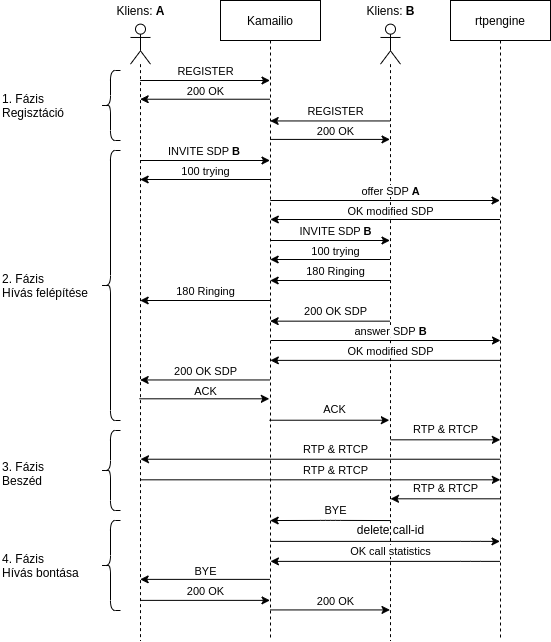
\includegraphics[width=0.9\textwidth, keepaspectratio]{figures/basic_call_flow.png}
	\caption{Kubernetes nélküli hívásfelépítés}
	\label{fig:callflow}
\end{figure}

Az \ref{fig:callflow} ábra segítségével a hívásfelépítés részeit.  Az ábrán látható 
egy teljes hívás folyamata a regisztrációtól egészen a hívás bontásáig. Négy részre 
bontottam a hívást annak érdekében, hogy könnyebb legyen a megértése.

Az első rész a regisztráció amelynek során a felhasználók csatlakoznak a SIP szerverhez.
Ilyenkor a kliens SIP REGISTER üzenetet küld a szervernek, amikkel hozzáadni, törölni és
lekérdezni lehet a felhasználó adait szerverről. Ha létezik a felhasználónak fiókja 
a szerveren, viszont még nem jelentkeztek be az adott eszközről akkor az első alkalommal 
egy 401 Unauthorized üzenettel tér vissza, ami felszólítja a klienst, hogy adja meg a 
hitelesítéshez szükséges felhasználói azonosítót és jelszót, amit egy újabb SIP REGISTER
üzenetben fog újraküldeni titkosítva. Ha minden megfelelt, akkor 200 OK üzenetet kap 
vissza a kliens, ami jelzi, hogy minden rendben és tud hívásokat kezdeményezni. Az ábrán
szereplő folyamat nem tartalmazza a 401-s üzenetet, mert már többször használva volt a 
kliens azon a virtuális gépen.

A következő rész pedig már a konkrét hívás kezdeményezése és felépítése. A hívást az 
\textbf{A} felhasználó kezdeményezi \textbf{B} irányába egy INVITE üzenettel, ami tartalmaz
egy SDP üzenetet is. Ez az SDP egy olyan protokoll, amivel a híváshoz kapcsolódó információkat
lehet továbbítani, mint például a támogatott média formátumok listája illetve a hívott fél
elérhetőségei. Mivel ebben az esetben \textbf{B} felhasználó címe létezik a szerveren így
a szerver 100 trying üzenettel jelzi \textbf{A}-nak, hogy elkezdte a hívást felépíteni. Erre
azért van szükség, hogy a kliens ne próbálkozzon újra a hívás felépítésével.

A szerver ilyenkor küld egy \textbf{offer} üzenetet az rtpengine felé, aminek legalább 
tartalmaznia kell az \textbf{A} által küldött SDP üzenetet, hívásazonosítót és a SIP üzenet
From mezőjét, ami az \textbf{A} azonosítója. Erre az rtpengine egy módosított SDP üzenetet küld
vissza a szervernek, amiben módosítja a cél címet és portot a sajátjára. Így minden RTP
üzenet elsőnek az rtpengine-hez fog elmenni és majd onnét megy tovább \textbf{B}-nek.

Ha ez is sikeresen megtörtént, a szerver átveszi a hívás kezdeményező szerepét a \textbf{B}-vel
szemben. Szóval küld egy INVITE üzenetet neki, amiben szerepel \textbf{A} azonosítója, de
a csatlakozást leíró mező az rtpengine címe lesz. A trying üzenet ebben az esetben is 
ugyan azt jelenti, mint mikor az \textbf{A} kezdeményezett. De itt már szerepel a 
\textbf{180 ringing}, amivel lehet jelzi, hogy feldolgozásra került az INVITE. Majd ugyan ez 
az üzenetet megkapja \textbf{A} is. 

Ha \textbf{B} elfogadta a hívást, akkor \textbf{200 OK}-l jelez a szervernek, amiből a
SIP szerver tudja, hogy \textbf{answer}-t kell küldenie az rtpengine felé, amivel a hívás teljesen
ki fog épülni az rtpengine-ben is. Az answer igazából ugyanazt a funkciót valósítja meg,
mint az offer. Mivel az rtpengine kapott offer-t és answer-t is, így a hívást kiépítheti
és az előzőleg lefoglalt négy porton képes fogadni a forgalmat, amit feldolgozva 
tovább küld. Azért foglal le négy port, mert felenként kell egy páros számú port az 
RTP forgalomnak és egy páratlan számú az RTCP-nek. Végül pedig egy SIP ACK üzenettel van
értesítve mind a két fél arról, hogy a hívás sikeresen kiépült és elkezdhetnek 
beszélni. 

Mivel már létezik a hívás így már lehet küldeni a forgalmat az rtpengine adott 
portjaira. Ahol a legegyszerűbb esetben annyi történik, hogy az \textbf{A}-hoz rendelt
RTP porton kapott csomagokat kiküldi a \textbf{B}-hez a hozzárendelt portról. Ugyanez
történik RTCP esetében is. 

Mikor vége a hívásnak, akkor megkezdődik a hívás lebontása egy BYE SIP üzenettel. Aminek
hatására a SIP szerver egy delete üzenetet ad ki az rtpengine felé, ami tartalmazza a hívás
azonosítóját. Ekkor törlődik minden a híváshoz kapcsolódó információ és a számukra kinyitott
portok is lezárnak. De a rtpengine válaszában szerepelnek a hívásról információk, amik alapján
könnyen lehet statisztikákat készíteni például a hívások átlagos hosszáról vagy minőségéről.